\documentclass[11pt]{article}
\usepackage{graphicx}
\usepackage{hyperref}
\usepackage{natbib}
\usepackage{amsmath}
\usepackage{dirtytalk}

\setlength{\textwidth}{6.5in}
\setlength{\headheight}{0in}
\setlength{\textheight}{8.0in}
\setlength{\hoffset}{0in}
\setlength{\voffset}{0in}
\setlength{\oddsidemargin}{0in}
\setlength{\evensidemargin}{0in}

\newcommand\tab[1][.5cm]{\hspace*{#1}}

\title{2D Ising Model}
  
\author{Billy Chan, Kim Mishra, Javan Tahir, Tenzin Tsega}

\begin{document}

\maketitle

\abstract{
This project focused on Monte Carlo sampling to create multiple 2D Ising models. Each model was created using Python programming in which we integrated the well-known Metropolis algorithm. By modifying the algorithm and appending extra functions, we were able to analyze the effects of varying the temperature, external magnetization, and initial spin condition. The dependency of the system energy and magnetization were plotted as a function of temperature for the various aforementioned conditions. The behavior of the energy and the magnetization fraction of the system as a function of temperature were consistent with our predictions.
}

\section{Introduction}
\label{sec:intro}
\tab In statistical mechanics, an ideal system treats particles such that they do not exert any significant force between each other. However, this project was concerned with predicting and analyzing the behavior of a non-ideal system. The 2D-Ising model is an example of a non-ideal system and was the focus of the experiment.

The premise of the model is that, by using Python programming, we were able to construct a square lattice representation of interacting magnetic dipoles. The model was assumed to be ferromagnetic which meant that magnetic dipoles favorably orient themselves in the same direction as their neighboring dipoles. Generally, dipoles exist in magnetic domains where all dipoles would be aligned for a given domain. Ferromagnets, like our model, may have many of these magnetic domains which can point in opposing directions. We can expect that taking the average of these domains yield a net magnetization of zero. However, dropping the temperature of the system low enough can push the system to cause the dipoles to align. Similarly, heating an aligned system initially in a low temperature environment should remain well-aligned until its Curie temperature is reached and a phase transition occurs.

We were able to simulate this model by expanding upon the Metropolis algorithm. The algorithm is a type of Monte Carlo simulation, which utilizes iterative random sampling to obtain results. The motivation for this project was to analyze how the energy and magnetization of a system as a function of temperature, behaved under a set of various conditions. For example, the effects of an external magnetic field or the effects of initial spin orientation.

When determining the total energy of the system as a function of temperature, each neighbouring pair of atoms contributed to the total energy of the system. It was defined by the following, where $s_i$ was the dipole of interest and $s_j$ was a neighbor in either the horizontal or vertical direction:
\[E= -J s_{i}s_{j}\]

Because we were also interested in magnetization, it was convenient to make the comparison between our simulation and an analytical result. Hence the analytical form for the magnetization as a function of temperature was defined as:
\[M(T) =
  \begin{cases}
                                   0 & \text{if $T>T_{c}$} \\
  \frac{(1+z^{2})^{1/4} (1-6z^{2}+z^{4})^{1/8}}{\sqrt{1-z^{2}}} & \text{if $T<T_{c}$}
  \end{cases}\]

\section{Methods}
\label{sec:methods}

\subsection{Rescaling the problem}
\label{sec:formulation}
\tab In order to perform the numerical analysis, we rescaled the problem so that we would only need one physical constant.  As such, all of our results were in terms of $T \cdot\frac{k_b}{J}$. In addition to this, $J$ and $k$ were set to 1 for convenience, yielding temperature results in Kelvin.

\subsection{Computational methods}
\label{sec:computational}
\subsubsection{Implementation}
\tab To implement the 2D Ising model, we first created an object (\textit{ising2D.py}) that initialized an $N \times N$ grid of magnetic moments. The object was given a set of initial conditions to choose from, assuming either a fully aligned system of dipoles or one with randomly assigned dipole spins. Every lattice point in the grid contained a spin which assumed an integer value of $-1$ or $1$ corresponding to spin up or spin down respectively:

\[s \in \{-1,1\}\] 

Even though the 2D Ising model was a square lattice representation, we were able to make a topological transformation using modular algebra. This was accomplished in order to apply periodic boundary conditions in both the horizontal and vertical directions, effectively reducing the topology of the model to a torus.

To simulate the behavior of the spin system, we used Markov Chain Monte Carlo methods (MCMC). The process was as follows: we initially chose an arbitrary dipole to flip. We then considered the energy it would take to flip it for which it was successful if the change in system energy was either negative or remained the same. If the system energy increased though, we used the Boltzmann condition to determine whether the flip would be accepted or rejected. Whether the dipole was flipped or not, we then proceeded to repeat this process until every dipole had several chances to be flipped. The \textit{.run()} method in our object performed this operation for a specified number of steps in order for the system to converge to a steady state. The \textit{ising2D} object included a method, \textit{.changingTemp()}, to analyze the behaviour of the system as we varied the temperature, which ran the MCMC simulation at each temperature point and recorded the steady state magnetization and energy. The steady state of the system at one temperature step was used as the initial state for the following step. 

\subsubsection{Markov Chains and the Metropolis-Hastings Algorithm}
\tab Much of this section follows the treatment as described by Newman\cite{Newman} closely. For any physical system at constant temperature, the probability of occupying a particular energy state, $E_i$, is given by the Boltzmann distribution:

\[P(E_{i}) = \frac{e^{-\beta E_i}}{Z}\]
where $\beta = 1/k_B T$ and $Z$ is the partition function: 
\[Z = \sum_j e^{-\beta E_j}\]

If all possible energy states were known, one could compute the partition function and the expectation values for any number of observable quantities. In the simulation setting, however, the energy states are not necessarily known. Thus, in order for our system to occupy energy states in accordance with Boltzmann statistics, we will need to be more clever. The solution is to evolve our system from time step to time step as a Markov Chain. As suggested by its name, a transition from state $i$ to state $j$ must obey the Markov property. That is, the immediate future of the system is determined only by the present. Each transition from state $i$ to state $j$ is assigned a transition probability $T_{ij}$. By choosing these transition probabilities correctly, we can force the system to obey Boltzmann statistics. In particular, the transition probabilities should be normalized: 

\[\sum_j T_{ij} = 1\]
In addition, we can choose the transition probabilities to obey: 
\[\frac{T_{ij}}{T_{ji}} = \frac{P(E_j)}{P(E_{i})} = \frac{e^{-\beta E_j}/Z}{e^{-\beta E_i}/Z}\]
so that the partition function conveniently cancels. We can also prove that the Boltzmann distribution is a fixed point of the Markov Chain. Suppose the probability of being in the ith state in the Markov Chain is already given by the Boltzmann distribution. Then the the probability of being in state j in the successive step of the chain is given by the sum over all paths leading to j:

\[\sum_i T_{ij} P(E_i) = \sum_i T_{ji}P(E_j) = P(E_j)\sum_i T_{ji} = P(E_j)\]
where have made use of the normalization and the ratio of transition probabilities given above. Thus if we have a Boltzmann distribution over states at some step in the chain, we will remain with a Boltzmann distribution over future states.

Our choice for the transition probabilities align with the famous Metropolis-Hastings algorithm. At one step in the simulation, we randomly select a spin and flip it. If this move lowers the energy of the system, we unconditionally accept it based on the principles of minimum energy. If the move raises the energy of the system, the acceptance is determined by what we will call the Boltzmann condition. Furthermore the move is accepted with a probability of the Boltzmann factor $e^{-\beta(E_j - E_i)}$. The probabilities are summarized as follows:

\[P(a) = 
\begin{cases}
1 & \text{if $E_j \leq E_i$ }\\
e^{-\beta(E_j - E_i)} & \text{if $E_j > E_i$}
\end{cases}
\]
By utilizing these conditions in our simulation, we were able satisfy the proper ratio of transition probabilities.

To cut down on run-time, our program did not recalculate the energy for every move. Instead, we simply calculated the energy contribution from the randomly selected lattice atom before and after the flip. If the move was accepted, we added the difference $E_f - E_i$ to the total energy of the system which was just an attribute of the object. If the move was rejected, we flipped the spin back to its previous state and did not update the energy of the system.

To attain steady state, we estimated that there should have been at least $N^2$ steps in the simulation (since there were $N^2$ lattice points to work with). This ensured that there was a reasonable possibility for each spin to have been flipped in the simulation. We used 2500 steps in all simulations to account for the possibility of altering the same spin more than once. We also ran simulations with up to 500,000 steps and noticed no difference in the standard deviation of the energy or magnetization as compared to 2,500 steps. This was another method to ensure the integrity of the results.

\section{Results and Discussion}
\label{sec:results}

\begin{center}
    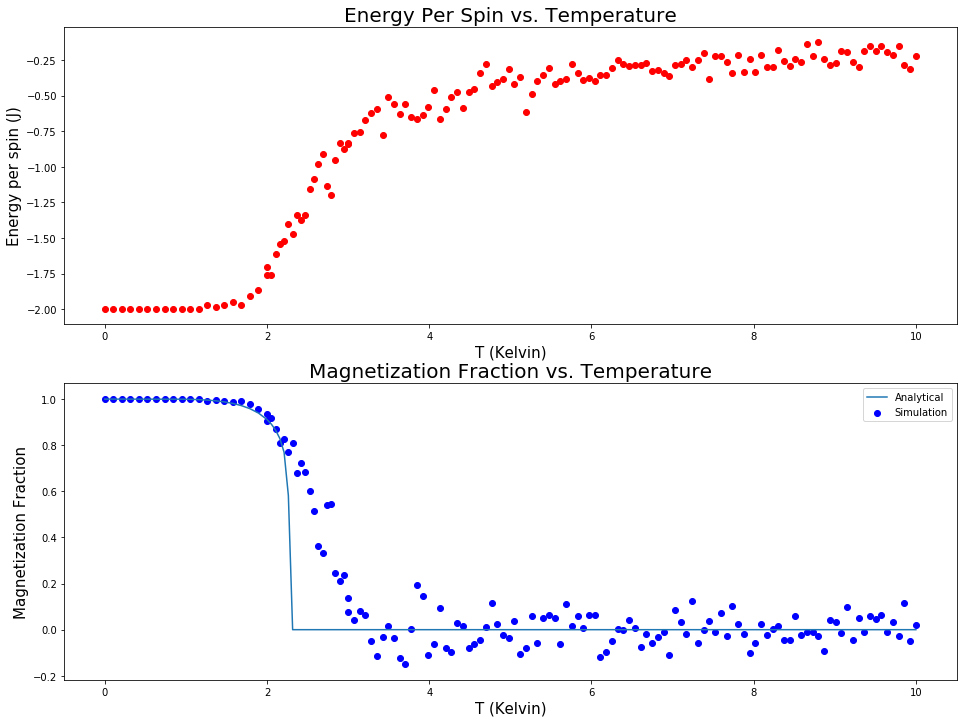
\includegraphics[width = \linewidth]{alignedspinNoField.png}
    \caption{\textbf{Figure 1: Heating of initially aligned spins under the effects of no external magnetic field, H = 0J.}}
    \label{fig:plt1}
\end{center}

One can perform the energy sums analytically to confirm that the energy contribution of each spin for a fully aligned lattice is indeed -2. This supported the energy curve shown in the plot [Figure 1]. In addition, the system began fully aligned such that it had magnetization 1. As the temperature increased, we initially saw very little change in both plots. However, as we passed the Curie temperature ($T_C \approx 2.3$) the magnetization and energy curves began to change. With increasing temperature, thermal fluctuations caused an increase in the likelihood of accepting an energetically unfavorable move thereby causing the spins to decohere. The analytical prediction for the magnetization was plotted alongside the simulation. While theory and simulation agreed for low temperatures and high temperatures, we observed that the rate of the transition for the simulation was a bit slow. This was attributed to the nature of the constructed lattice such as its finite size.

The slope of the energy versus temperature graph was significant. To elaborate, this slope was the heat capacity of the system, thereby meaning that more work was necessary to raise the temperature. This was evident as the phase transition occurred, since the system wants to remain in its aligned state with the maximal energy stored. Theory predicts that the sharp change in energy should lead to a discontinuity in the heat capacity, at the point of inflection, suggesting a phase transition in the system from fully aligned to disordered. Because our slope was not as drastic, we saw a smooth transition from order to disorder. 

\begin{center}
    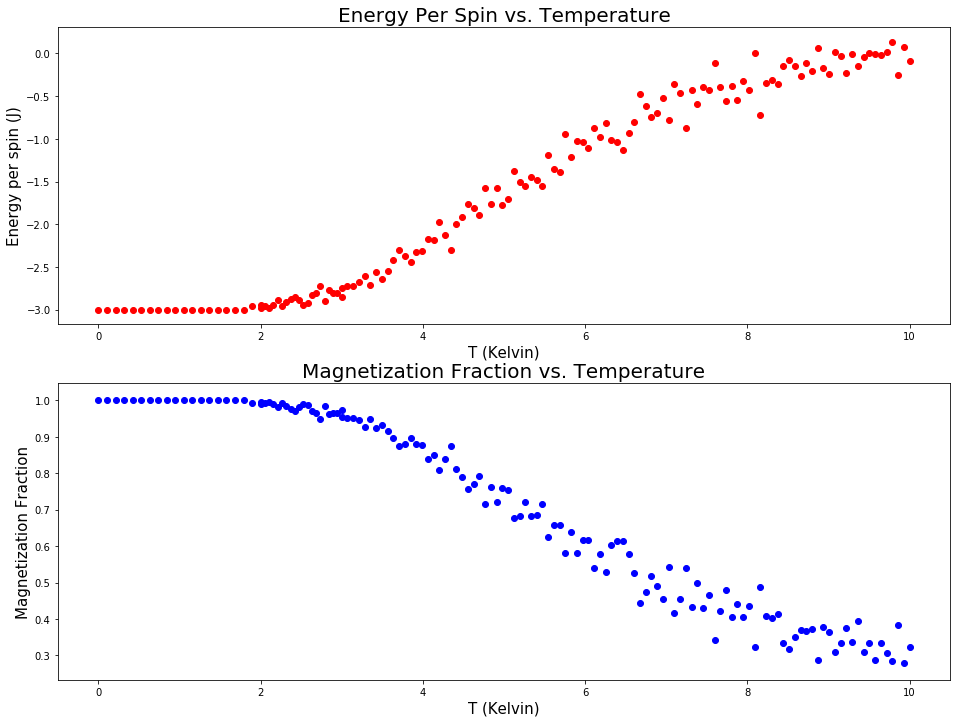
\includegraphics[width = \linewidth]{alignedPosField.png}
    \caption{\textbf{Figure 2: Heating of initially aligned spins under the effects of a positive external magnetic field, H = 2J.}}
    \label{fig:plt1}
\end{center}

The plot [Figure 2] confirmed our prediction, that the magnetic field should resist the system's tendency to have zero magnetization. In comparison to [Figure 1], this was evident by just observing the plots' slopes and convergence temperatures. As opposed to no field, the positive field created a force which kept the dipoles from flipping. When the temperature kept increasing well beyond the Curie temperature, the thermal fluctuations became large enough to combat the magnetic field thereby allowing the magnetization to converge (at a rate proportional to the field strength).

\begin{center}
    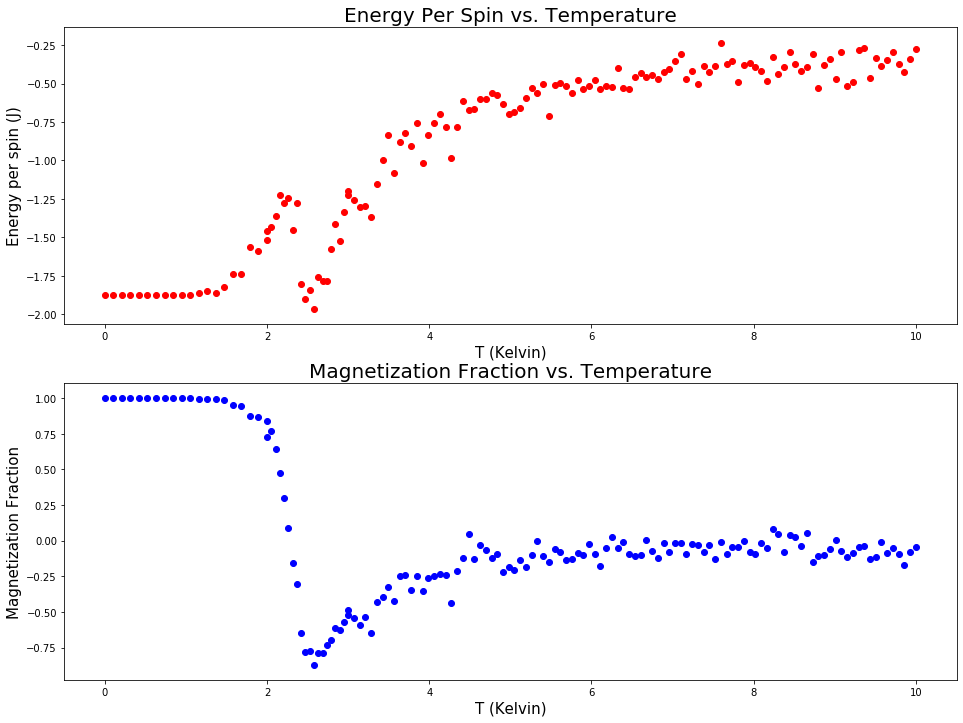
\includegraphics[width = \linewidth]{alignedNegField.png}
    \caption{\textbf{Figure 3: Heating of initially aligned spins under the effects of a strong negative external magnetic field, H = -0.25J.}}
    \label{fig:plt1}
\end{center}

Notice that the energy [Figure 3] was raised, lowered, and then raised again. Consider that this was due to the thermal effects and the external magnetic field. The initial raising of the energy was caused by the Curie temperature being met, in which the domains broke away from the initial spin configuration. With the spins being released from this configuration, the external magnetic field became dominant and aligned the spins to its field. As the temperature continued to rise, the energy approached zero since the spins would also become less susceptible to the field. The magnetization saw a drop from 1 to -1, which makes sense since the spins aligned with the external field past the Curie temperature. The magnetization data supported the energy data beyond this point in that they both tended to zero, as the spins became increasingly randomly oriented with the rising temperature.

\begin{center}
    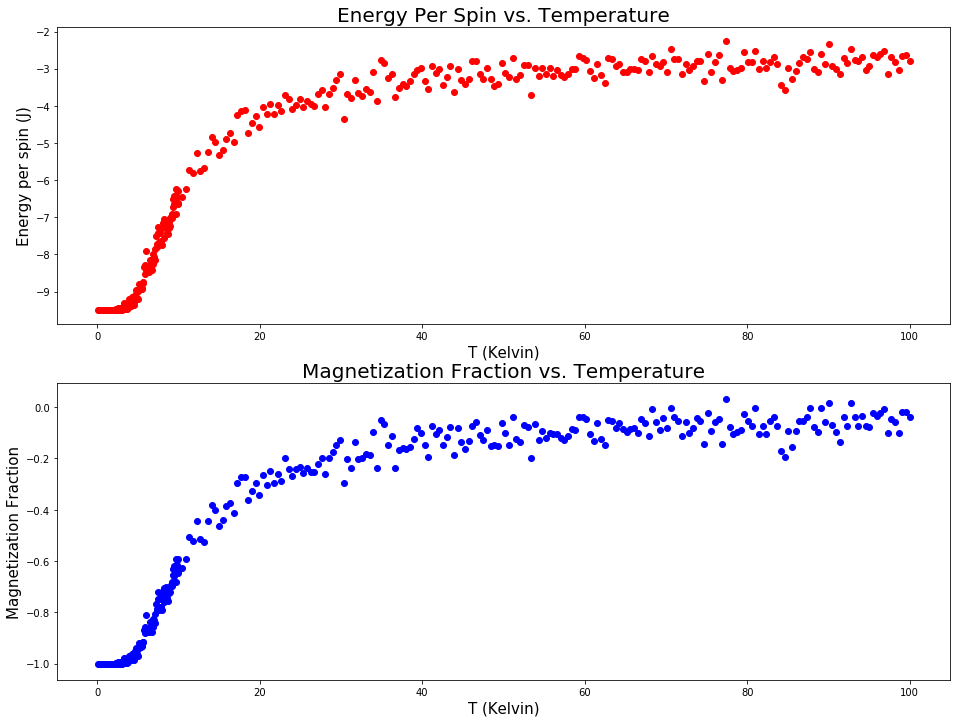
\includegraphics[width = \linewidth]{alignedNegFieldStrong.png}
    \caption{\textbf{Figure 4: Heating of initially aligned spins under the effects of a weak negative external magnetic field, H = -5J.}}
    \label{fig:plt1}
\end{center}

The energy data [Figure 4] was expected, as the system practically immediately aligned with the external field due to its magnitude. The magnetization was similar in form for the same reason. This data differed from the weak field in that the system was hardly even given a chance for the spins to align in their initial all spin up state. As the temperature continued to rise though, we observed that the system behaved as expected since the spins would become more randomly oriented. This was supported by the fact that both the energy and magnetization tended to zero with increasing temperature.

\begin{center}
    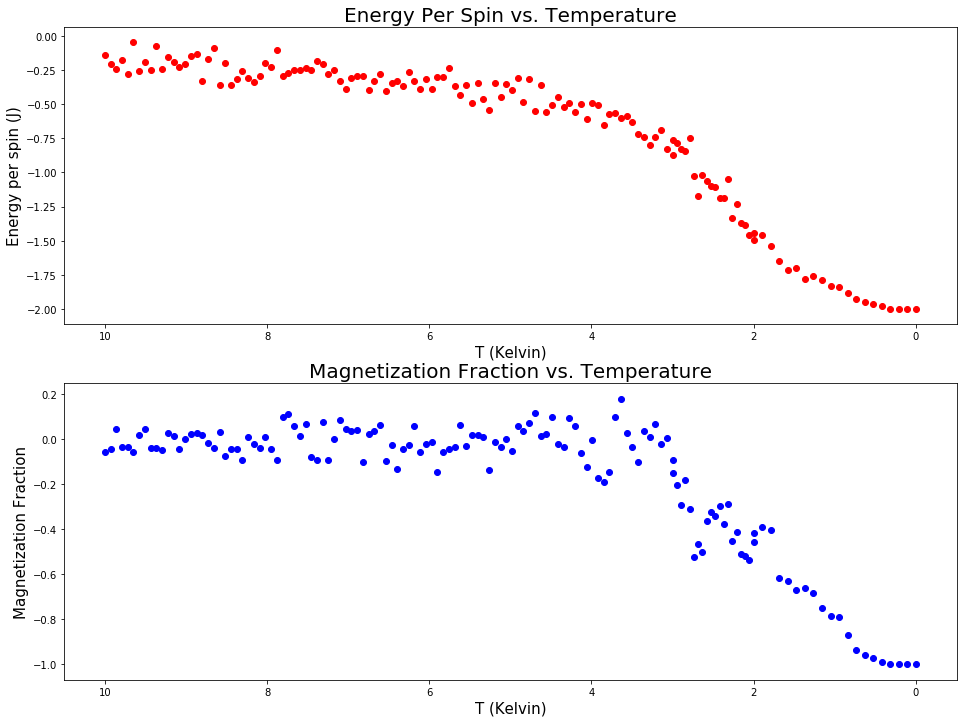
\includegraphics[width = \linewidth]{randomNoField.png}
    \caption{\textbf{Figure 5: Cooling of initially random spins under the effect of no external magnetic field, H = 0J.}}
    \label{fig:plt1}
\end{center}

We observed from the plots [Figure 5] that both the energy and magnetization of the system remained near the same values for most of the simulation. For the energy this was in a "low" energy state and for magnetization this was near zero. As the system cooled down, the energy dropped to about -2 and the magnetization became uniform to all spins down. These results were expected since the spins should have aligned as the temperature dropped. The system holds the most energy in the state where all spins are oriented in the same direction, and the magnetization tending to -1 was just a matter of probability. Because there was no external field present, the system may "choose" to either orient all spins up or all spins down. Hence we expected the magnetization to have either been 1 or -1 with equal probability.

\begin{center}
    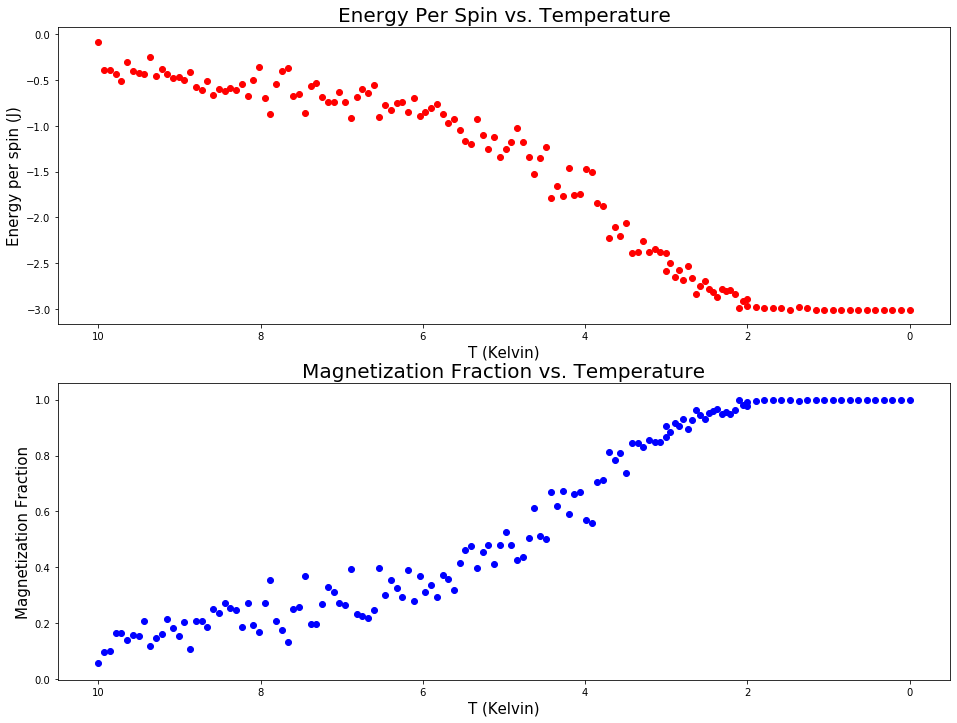
\includegraphics[width = \linewidth]{randomPosField.png}
    \caption{\textbf{Figure 6: Cooling of initially random spins under the effect of a positive external magnetic field, H = 1J.}}
    \label{fig:plt1}
\end{center}

We observed from the plots [Figure 6] that the system started off with energies and magnetization near zero. This was expected as spins were initialized to be random, with many of the dipoles cancelling each other out. As the temperature cooled down, the energy dropped to -3 and the spins became oriented to all point up. This was also reasonable since there was an external magnetic field, helping to "push" the dipoles in the upright orientation. The magnetization converged to a point that was proportional to the strength of the external positive field. The magnetic spins eventually all aligned in the direction of the external field, when the temperature became sufficiently low enough.

\begin{center}
    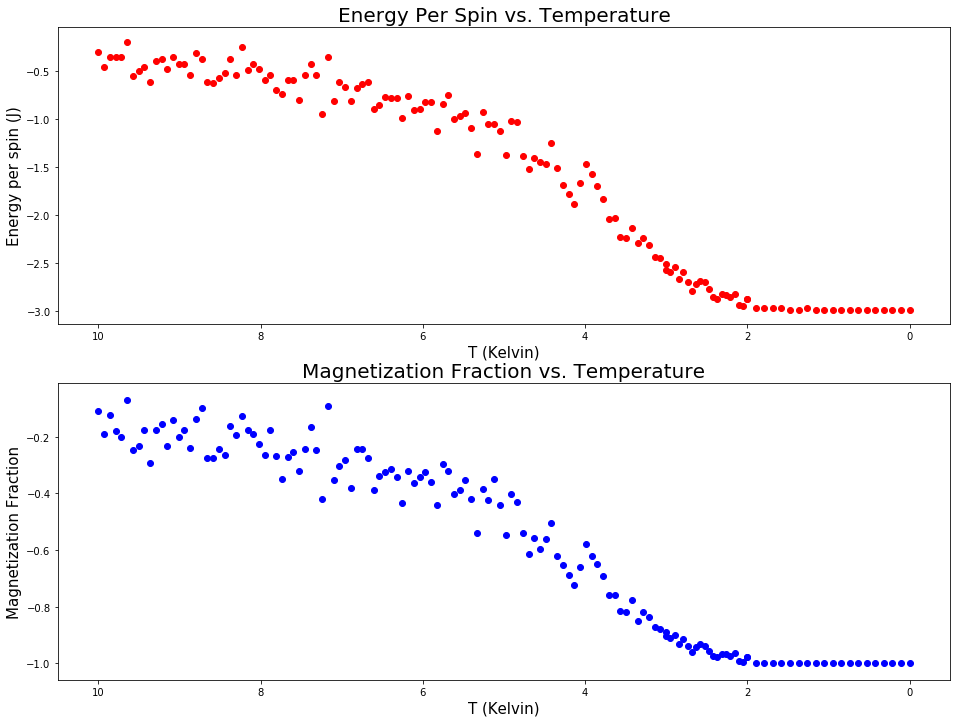
\includegraphics[width = \linewidth]{randomNegField.png}
    \caption{\textbf{Figure 7: Cooling of initially random spins under the effect of a negative external magnetic field, H = -1J.}}
    \label{fig:plt1}
\end{center}

We observed that the plots [Figure 7] for energy and magnetization both had similar initial conditions, starting near zero, and also had similar shapes as the temperature decreased to zero. As we cooled the system, it became entropically ordered, meaning the system became negatively magnetized as we would expect under the presence of a negative external field. We observed that the energy eventually converged as expected, with the dipoles all orienting themselves downwards. The energy converged to a value of -3. Note that this was higher (in magnitude) than the energy for the aligned spins without a field. This was because the energy contribution from the field was positive, pushing the equilibrium energy to a slightly higher value.

\section{Conclusion}

The Ising model served as a simplified representation of a ferromagnetic (or even anti-ferromagnetic) system. Using the Metropolis algorithm for Markov Chain Monte Carlo simulations, we implemented the Ising model on a two dimensional lattice. Despite its relative simplicity, the Ising model captures key features of the physical system, namely behavior above or below the Curie temperature. Of course we accepted experimental error, within reason, as these simulations are entirely dependent on the probabilistic nature of the Monte Carlo steps. If we had more powerful computers and time to work with, it would be trivial to just extend the dipole matrix or add more steps to the simulations. One could also refine this work by accounting for interactions beyond nearest neighbors. In particular, it would be interesting to use an interaction kernel that falls off with distance like true dipole interactions. This would, however, eliminate the simplicity that has made the Ising model so famous to begin with. In future trials of this project, it would also be worth considering graphic representations of the lattice as a function of temperature. One would easily be able to observe how the dipoles form and break magnetic domains over a range of temperatures.

\begin{thebibliography}{10}

\bibitem{Hocky}Hocky, Glen. "Metropolis Monte Carlo for the Ising Model" NYU Chemistry: Hocky Research Group. 2019. Available at \url{http://hockygroup.hosting.nyu.edu/exercise/ising-1d.html}

\bibitem{Princeton} \say{Introducing the Monte Carlo technique.} Princeton Univerity Physics. Fall 2014. Available at \url{http://physics.princeton.edu/~phy209/week5/index.html}

\bibitem{wiki} \say{Ising Model.} Wikipedia: The Free Encyclopedia. Wikimedia Foundation, Inc. 22 July 2004. Web. 3 Dec. 2019, \url{https://en.wikipedia.org/wiki/Ising_model}

\bibitem{Newman} Newman, Mark E. J. \emph{Computational Physics.} Createspace Independent Pub, 2012

\bibitem{Ludwig} Ridderstolpe, Ludwig. \emph{Exact Solutions of the Ising Model.} 
Uppsala University, Department of Physics and Astronomy, Division of Theoretical Physics. September 7, 2017. Available at \url{https://uu.diva-portal.org/smash/get/diva2:1139470/FULLTEXT01.pdf}

\bibitem{Schroeder} Schroeder, Daniel V. \emph{An Introduction to Thermal Physics.} San Francisco, CA: Addison Wesley, 2000.

\bibitem{RajGithub} Singh, Rajesh. "Ising Model" Available at \url{https://rajeshrinet.github.io/blog/2014/ising-model/}

\bibitem{Stack Overflow} https://stackoverflow.com/questions/2051744/reverse-y-axis-in-pyplot

\end{thebibliography}

\end{document}
